%%%%%%%%%%%%%%%%%%%%%%%%%%%%%%%%%%%%%%%%%%%%%%%%%%%%%%%%%%%%%%%%%%%%%%%%%%%%%%%
\subsection{Properties of the Bee Colony}
\label{subsec:colony}
%%%%%%%%%%%%%%%%%%%%%%%%%%%%%%%%%%%%%%%%%%%%%%%%%%%%%%%%%%%%%%%%%%%%%%%%%%%%%%%
Each snapshot consists of one component.
Table~\ref{tab:stats} summarizes the basic network properties for each snapshot.
The density $D$ is over 50\% for all snapshots.
The diameter $\langle d_{\texttt{max}} \rangle$ is three and the average shortest path length $\langle d \rangle$ is below two.
The global clustering coefficient $C_\Delta$ of all snapshots is higher than compared to an Erdös-Renyi random graph, averaged over 100 runs using the same number of nodes and edges.
The high clustering coefficient and the small diameter suggest a small-world network type.
On average, each bee is connected to at least 50\% of all other bees.

Figure~\ref{fig:fVSd} shows a positive correlation between the frequency of interactions and the total duration of interactions.
I chose the frequency of interactions as the weight for edges.
The edge weight distribution is shown in figure~\ref{fig:edgeWdist}.
Most edges have a low weight; only a few edges have a high weight.
It seems that bees do not prefer individuals bees for interaction.
Figure~\ref{fig:n3ageDist} shows the age distribution of the investigated snapshot 3. This distribution does not seem to follow any known distribution. It corresponds to the artificial tagging of bees. Consequently, bees of certain age groups are simply not present. The detection frequency of an individual bee is negatively correlated with its age (figure~\ref{fig:n3detfVSage}).

\begin{table}[htbp]
\small
\centering
\caption[Global network properties]{\textbf{Global network properties} $N$ number of nodes, $L$ number of links, $D$ diameter, $\langle d_{\texttt{max}} \rangle$ average path length, $\langle d \rangle$ diameter, $C_\Delta$ global clustering coefficient, $\langle k \rangle$ average degree and $\langle s \rangle$ represents the average strength, as introduced in section~\ref{sec:definitions}.}
\label{tab:stats}
\vspace*{5mm}
\begin{tabular}{rccccccccc}
\toprule
{} &  $N$ &   $L$ &  $D$ &  $\langle d_{\texttt{max}} \rangle$ &  $\langle d \rangle$ &   $C_\Delta$ & $\langle k \rangle$ &  $\langle s \rangle$ \\
\midrule
Snapshot 1 & 922 & 291179 & 0.69 & 3 & 1.32 &  0.79 & 631.62 & 5680.17 \\
Random 1  & 922 & 291179 & 0.69 & 2 & 1.31 &  0.69 & 631.62 & - \\ \midrule
Snapshot 2 & 978 & 256066 & 0.54 & 3 & 1.46 &  0.72 & 523.65 & 3977.94 \\
Random 2  & 978 & 256066 & 0.54 & 2 & 1.46 &  0.54 & 523.65 & - \\ \midrule
Snapshot 3 & 922 & 259421 & 0.61 & 3 & 1.39 &  0.75 & 562.74 & 4205.99 \\
Random 3  & 922 & 259421 & 0.61 & 2 & 1.39 &  0.61 & 562.74 & - \\
\bottomrule
\end{tabular}
\end{table}

\begin{figure}[htb]
	\centering
	\begin{subfigure}[b]{0.49\textwidth}
	\centering
	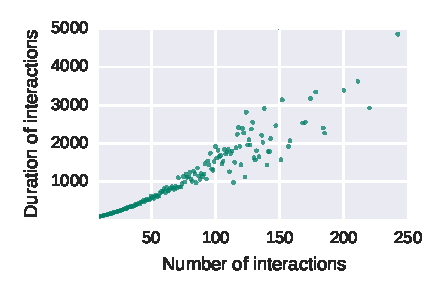
\includegraphics[width=1.0\textwidth]{Figures/n3-freqVSduration}
	\caption[Type of edge weights]{Type of edge weights}
	\label{fig:fVSd}
	\end{subfigure} 
	\begin{subfigure}[b]{0.49\textwidth}
	\centering
	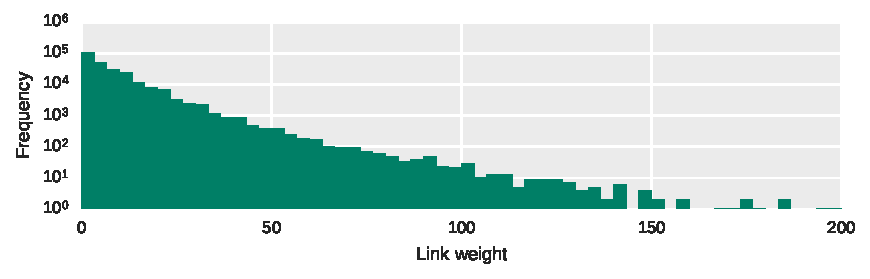
\includegraphics[width=1.0\textwidth]{Figures/n3-edgeWeightDist.pdf}
	\caption[Edge weight distribution]{Edge weight distribution}
	\label{fig:edgeWdist}
	\end{subfigure}
	\caption[Edge wights]{\textbf{Edge wights} (a) Correlation between number of interactions and total duration of interactions. The number of interactions is chose as the edge weight. (b)  The edge weight distribution decays exponentially.}
	\label{fig:edges}
\end{figure}

\begin{figure}[htb]
	\centering
	\begin{subfigure}[b]{0.33\textwidth}
	\centering
	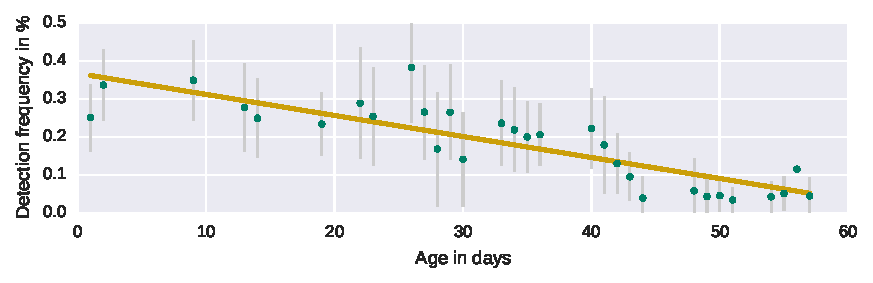
\includegraphics[width=1.0\textwidth]{Figures/n3_detFvsAge}
	\caption[Correlation]{Correlation}
	\label{fig:n3detfVSage}
	\end{subfigure} 
	\begin{subfigure}[b]{0.66\textwidth}
	\centering
	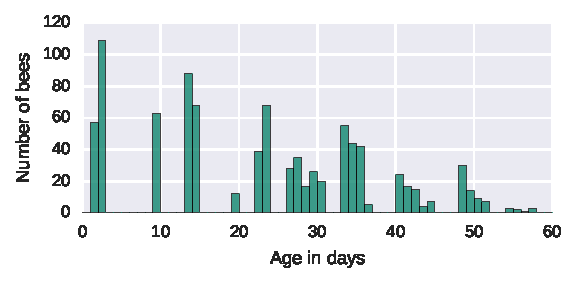
\includegraphics[width=1.0\textwidth]{Figures/n3_ages.pdf}
	\caption[Age distribution]{Age distribution}
	\label{fig:n3ageDist}
	\end{subfigure}
	\caption[Age distribution and correlation with detection frequency of snapshot~3]{\textbf{Age distribution and correlation with detection frequency of snapshot~3} (a) Detection frequency and the age of a bee seem to be negatively correlated. (b) The age of bees ranges from one to 60 day, but some age groups are missing.}
	\label{fig:ageDetF}
\end{figure}